\chapter{Implementation}\label{implementation}
Das folgende Kapitel dokumentiert die wichtigsten Bestandteile der Implementation einer Testanwendung mit den betrachteten Frameworks. Dabei werden grundsätzliche Konzepte durch einfache Anwendungsfälle abgedeckt. Das Ziel sind nach Möglichkeit identische Webapplikationen, um die Vorgehensweise und Probleme vergleichen zu können. Sie hat nicht den Anspruch, alle erdenklichen Use-Cases abzudecken. Auf Drittbibliotheken- und Frameworks wird weitestgehend verzichtet. 
Der vollständige Quelltext ist auf GitHub zu finden\footnote{siehe: https://github.com/fschmeis/bthesis\_react\_angular}, im diesem Kapitel werden nur Ausschnitte abgebildet.

\section{Anforderungsbeschreibung}
Die Anwendung soll Rezepte und Zutaten verwalten und erfüllt genauer die folgenden Anforderungen:
\begin{enumerate}
  \item Rezepte können mit Namen und Anweisungen, benötigten Zutaten und Mengen eingetragen werden
  \item Es können neue Zutaten hinzugefügt werden
  \item Eine Übersicht zeigt die gespeicherten Zutaten und Mengen an
  \item Eine Übersicht zeigt Rezepte und gibt an, ob die geforderten Zutaten in ausreichender Menge vorhanden sind
\end{enumerate}

Die Applikation verfügt über 3 mit Tabs navigierbare Ansichten für die Anforderungen 1, 3 und 4. Die Eingabe der Zutaten erfolgt über einen Dialog. Über den Tabs liegt eine einfache Leiste mit dem Titel der Anwendung.

\subsubsection{Rezepte hinzufügen}
Der Nutzer kann im linken Bereich der Ansicht über ein Formular den Titel und die Anweisen des Rezeptes eingeben. Auf der rechten Seite ist ein Button, der beim Klick den Zutaten-Dialog öffnet. Die bereits hinzugefügten Zutaten werden darunter in einer Liste angezeigt.

Unter diesem Formular sind zwei Buttons angeordnet: Ein Button zum Speichern des Rezeptes, der andere zum Zurücksetzen des Formulars.

\subsubsection{Zutaten}
Der Nutzer sieht eine Tabelle der angelegten Zutaten mit Einheit und verfügbarer Menge. Über einen Button darüber öffnet sich der Zutaten-Dialog, dort können neue Zutaten hinzugefügt werden. Die Tabelle lässt sich sortieren und filtern.

\subsubsection{Kochbuch}
Hier werden die angelegten Rezepte seitenweise angezeigt. Links stehen Titel und Anweisungen, rechts eine Liste mit benötigten und vorhandenen Zutaten. Ist alles nötige vorhanden, dann werden mit Klick auf den Button "Kochen" die Mengen der verbrauchten Zutaten entsprechend reduziert.

Unter dem Rezept kann über Pfeile geblättert werden. Darüber ist einer Filterleiste, um nach bestimmten Rezepten zu suchen.

\subsubsection{Zutaten-Dialog}
Ein einfacher Dialog, der Zutatenname, Einheit und Menge abfragt. Mit dem Button \glqq Hinzufügen\grqq werden die Eingaben bestätigt, ein weiterer Button ermöglicht den Abbruch der Aktion.

\subsection{Umsetzung}
Die Umsetzung soll möglichst ohne Drittlösungen auskommen, um die möglichen Grenzen der Standard-Versionen aufzuzeigen. Aus den Material Design Frameworks Angular Material\footnote{siehe: https://material.angular.io} und Material UI (React) \footnote{siehe: https://material-ui.com} werden sowohl einfache Komponenten als auch Schriftarten und Themes übernommen. Letzteres besitzt deutlich mehr Komponenten, daher wird mit Angular begonnen. Für das Styling wird Sass verwendet.

\section{Angular}
\subsection{Dateistruktur}
Das Projekt wird in verschiedene Teilbereiche strukturiert. Die Hauptkomponente der Anwendung (\textit{app.component.html|ts|scss}) befindet sich automatisch direkt im \textit{app}-Ordner und beinhaltet den Einstiegspunkt der Anwendung. Unter \textit{app/components/} finden sich die 3 Hauptkomponenten der Anwendung. In einem weiteren Ordner (\textit{app/shared/components}) befindet sich die Dialog-Komponente. Der Dialog wird an zwei Stellen benötigt und es ist zur Übersicht sinnvoll, diesen Umstand schon in der Dateistruktur ersichtlich zu machen. Im \textit{shared}-Ordner befinden sich außerdem die Models und Services. 

Die Implementation in Angular mit den entsprechenden Vorüberlegungen unkompliziert. Das Angular CLI erzeugt automatisch neue Komponenten oder Services und fügt sie dem App-Modul hinzu. 

\subsection{Models}
Die Models bilden das grundlegende Datenmodell der Anwendung ab (Listing \ref{lst:listing18}). Unter \textit{Unit} werden die verfügbaren Einheiten (string) deklariert, die der Nutzer für Zutaten wählen kann. Eine Zutat \textit{Ingredient} definiert sich aus Name, Anzahl und Einheit, ein Rezept (\textit{Recipe}) aus Name, Anweisungen und Zutaten.

\begin{listing}
\caption{Datenmodell}
\label{lst:listing18}
\begin{minted}{ts}
// unit.enum.ts
export enum Unit {
  tl = 'TL',
  el = 'EL',
  stk = 'Stück',
  bnd = 'Bund'
  /* ... */
}
// ingredient.model.ts
export interface Ingredient {
  name: string;
  amount: number;
  unit: Unit;
}
// recipe.model.ts
export interface Recipe {
  name: string;
  instructions: string;
  ingredients?: Ingredient[];
}
\end{minted}
\end{listing}

\subsection{Services}\label{sssec:impl_services}
Die Anwendung besitzt zwei Services als Schnittstelle zum Backend, die mit dem HTTP-Client auf die Backend-API zugreifen. Die Services werden mit der beschriebenen Dependency Injection über den Konstruktor übergeben und können dann in den Komponenten genutzt werden. Im Listing \ref{lst:listing19} in der \inlinecode{OnInit}-Methode, die bei der Initialisierung der Komponente aufgerufen wird.

\begin{listing}
\caption{Verwendung der Services}
\label{lst:listing19}
\begin{minted}{ts}
// cookbook.component.ts
export class CookbookComponent implements OnInit {
  /* ... */
  constructor(
    private recipeService: RecipeService,
    private ingredientService: IngredientService,
    /* ... */
  ) {}

  public ngOnInit(): void {
    this.fetchData();
  }

  private fetchData(): void {
    this.recipeService.getRecipes().subscribe((recipes) => {
      this.recipes = recipes;
      this.currentRecipe = this.recipes[0];
    });

    this.ingredientService.getIngredients().subscribe((ingredients) => {
      this.storedIngredients = ingredients;
    });
  }
  /* ... */
}
\end{minted}
\end{listing}

\subsection{Komponenten}
Die Anwendung besteht aus 4 Komponenten. Die \textit{app}-Komponente ist die Hauptkomponente und Startpunkt der Anwendung. Sie enthält die Toolbar mit dem Anwendungstitel und eine Tab-Leiste, über welche die anderen Teilkomponenten erreicht werden können (Abbildung \ref{fig:kochbuch_angular}).

\subsubsection{Kochbuch}
\begin{figure}
  \centering
  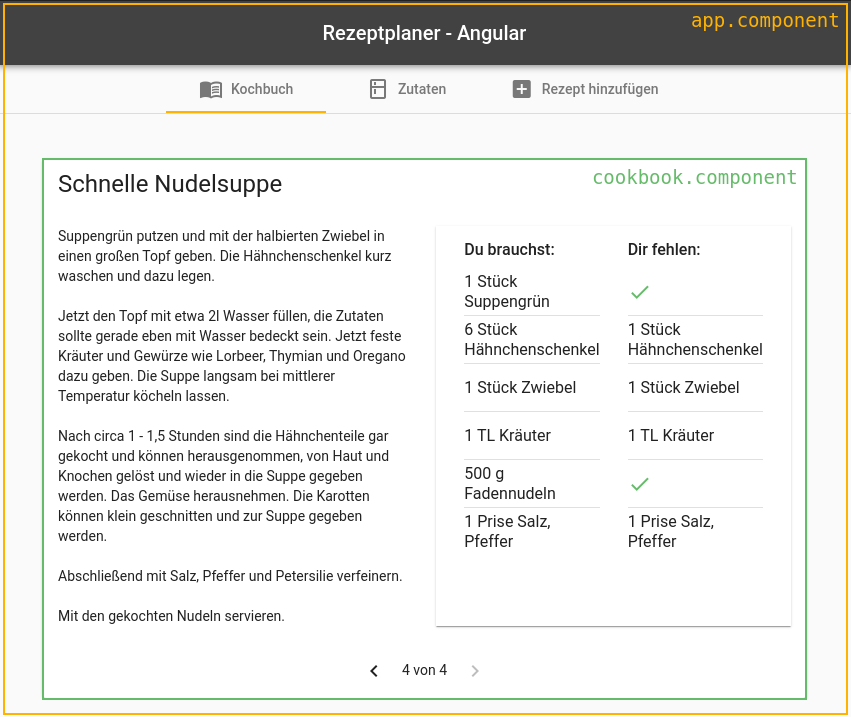
\includegraphics[scale=0.6]{Grafiken/03_Implementation/Kochbuch_Angular_edited.png}
  \caption{Kochbuch}
  \label{fig:kochbuch_angular}
\end{figure}

Die Komponente enthält neben der Service-Abfrage aus Listing \ref{lst:listing19} die ViewModel-Logik zum Vor- und Zurückblättern der Rezepte, zur Berechnung der fehlenden Zutatenmenge und Entnahme der Zutaten, wenn das Rezept gekocht wird. Die Template (Auszug im Listing \ref{lst:listing20}) definiert lediglich die Darstellung des ViewModels. Die mit \inlinecode{mat} beginnenden Tags referenzieren Komponenten der Material-Bibliothek. 

\begin{listing}
\caption{Template der Zutaten-Checkliste}
\label{lst:listing20}
\begin{minted}{html+ng2}
<div *ngIf="insufficientIngredients(); else cook">
  <span>Dir fehlen:</span>

  <mat-list role="list">
    <mat-list-item role="listitem"
      *ngFor="let ing of currentRecipe.ingredients; last as isLast">

      <ng-container *ngIf="getMissingAmount(ing) > 0; else tick">
        {{getMissingAmount(ing)}} {{ing.unit}} {{ing.name}}
      </ng-container>

      <ng-template #tick>
        <mat-icon id="tick">done</mat-icon>
      </ng-template>

      <mat-divider *ngIf="!isLast"></mat-divider>

    </mat-list-item>
  </mat-list>
</div>

<ng-template #cook>
  <div id="cook">
    <button mat-raised-button color="primary"
      (click)="cookRecipe()">Kochen
    </button>
  </div>
</ng-template>
\end{minted}
\end{listing}

In Zeile 6 wird mit \inlinecode{ngFor} über alle Zutaten des aktuellen Rezeptes iteriert, für jede dieser Zutaten wird ein neues \inlinecode{mat-list-item} erzeugt, welches entweder Text (fehlende Menge, Einheit und Zutat) oder ein Häkchen-Icon enthält. Bestimmt wird das durch die Abfrage in Zeile 8, sind genug Zutaten vorhanden, dann wird die Template-Variable \inlinecode{tick} wahr und das Icon gerendert. \inlinecode{ng-template} und \inlinecode{ng-container} sind strukturelle Direktiven, die selbst nicht gerendert werden.

\subsubsection{Zutaten}
\begin{figure}
  \centering
  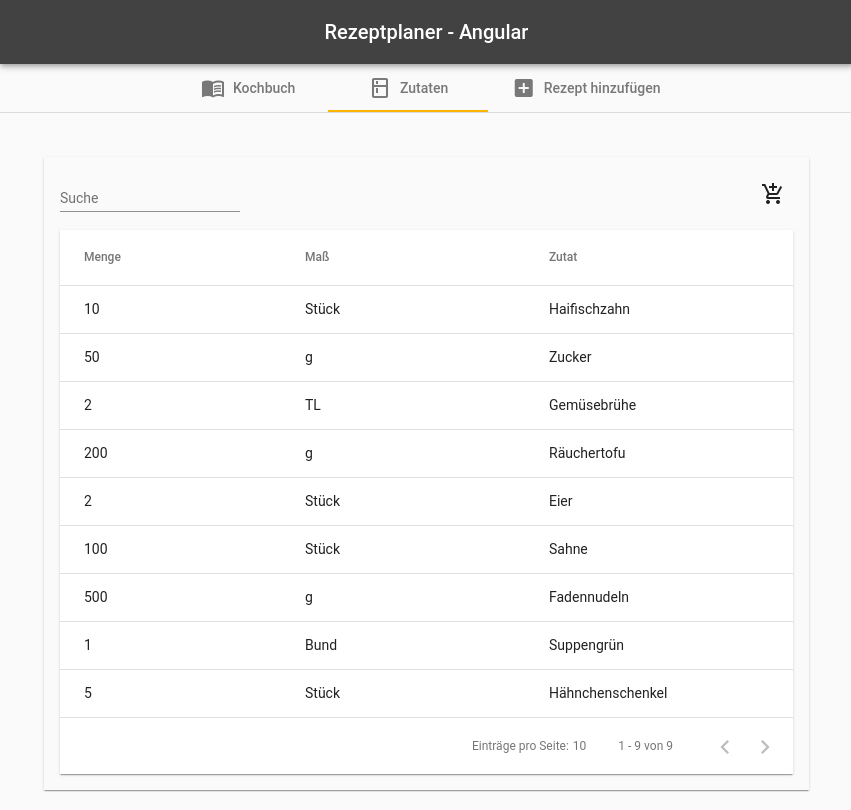
\includegraphics[scale=0.5]{Grafiken/03_Implementation/Zutaten_Angular.png}
  \caption{Zutaten-Übersicht}
  \label{fig:zutaten_angular}
\end{figure}

Die Übersicht der vorhandenen Zutaten besteht aus einer Tabellenkomponente der Material-Bibliothek und einem Button, der den Zutaten-Dialog öffnet. Die Material-Tabelle verfügt über die Möglichkeit, Spalten zu sortieren und durch Einträge zu schalten. Eingaben in der Suchleiste filtern die Datenquelle (Listing \ref{lst:listing21}).

\begin{listing}
\caption{Setzen und Filtern der Datenquelle}
\label{lst:listing21}
\begin{minted}{ts}
export class IngredientsComponent {
  dataSource!: MatTableDataSource<Ingredient>;
  /* ... */
  private fetchIngredients(): void {
    this.ingredientService.getIngredients().subscribe((ingredients) => {
      this.dataSource = new MatTableDataSource(ingredients);
    });
  }
  /* ... */
  public applyFilter(event: Event): void {
    const filterValue = (event.target as HTMLInputElement).value;
    this.dataSource.filter = filterValue.trim().toLowerCase();

    if (this.dataSource.paginator) {
      this.dataSource.paginator.firstPage();
    }
  }
}
\end{minted}
\end{listing}

\subsubsection{Rezepte hinzufügen}
\begin{figure}
  \centering
  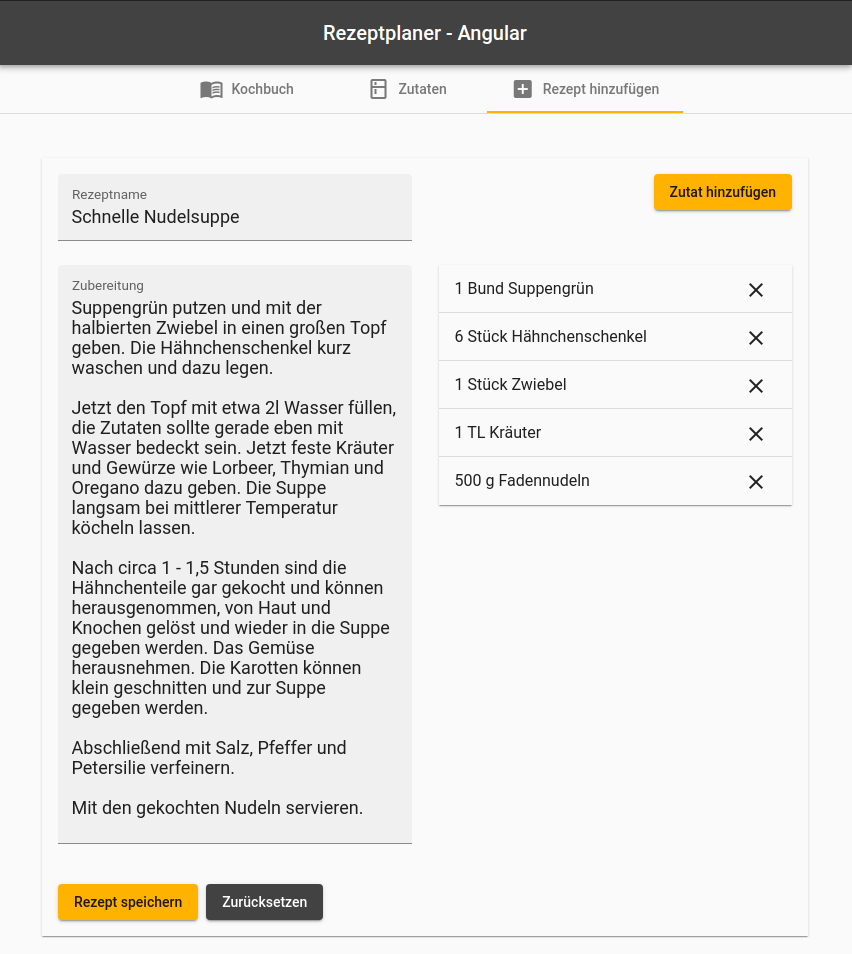
\includegraphics[scale=0.5]{Grafiken/03_Implementation/Hinzufuegen_Angular.png}
  \caption{Rezepte hinzufügen}
  \label{fig:hinzufuegen_angular}
\end{figure}

Die Komponente definiert Methoden, die das Formular zurückzusetzen, Zutaten hinzuzufügen oder entfernen und das Rezept bei entsprechender Nutzereingabe zu speichern.

\subsubsection{Zutaten-Dialog}
\begin{figure}
  \centering
  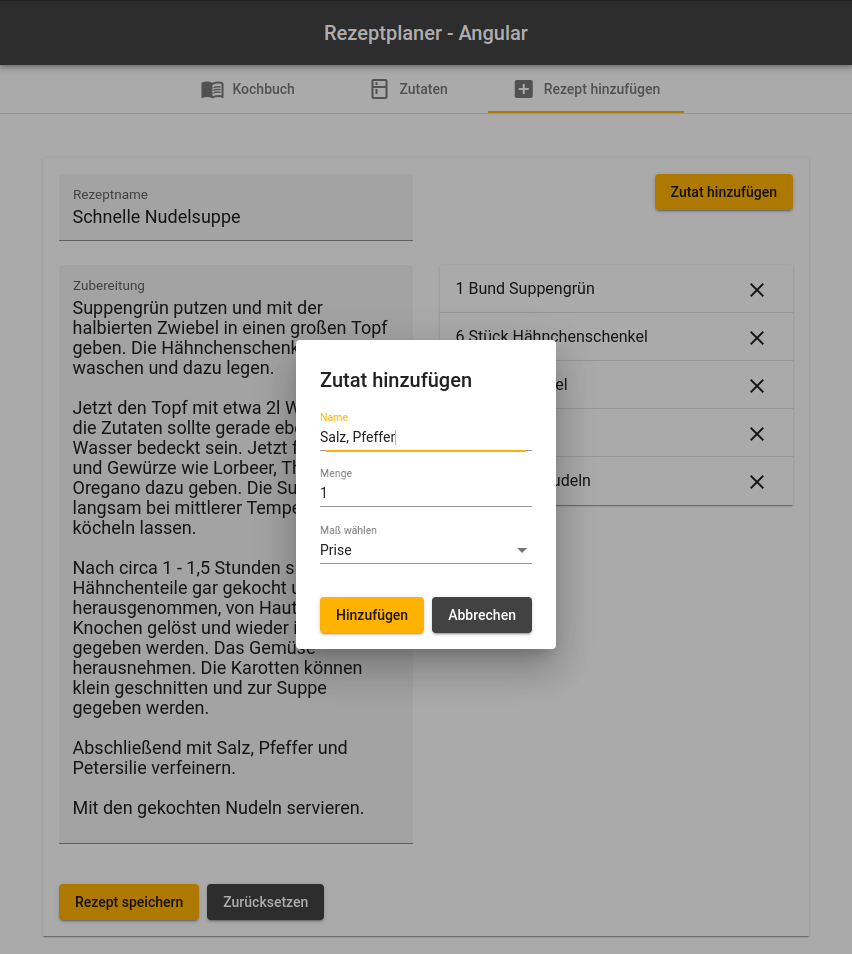
\includegraphics[scale=0.5]{Grafiken/03_Implementation/Dialog_Angular.png}
  \caption{Zutaten-Dialog}
  \label{fig:dialog_angular}
\end{figure}

Der Dialog wird aus anderen Komponenten heraus aufgerufen. Mit Angular Formularen lassen sich die eingegeben Werte validieren. Das Ergebnis des Dialogs wird im Anschluss wieder an die aufrufende Komponente zurückgegeben (Listing \ref{lst:listing22}).

\begin{listing}
\caption{Dialogaufruf und Rückgabe der Daten}
\label{lst:listing22}
\begin{minted}{ts}
// add-recipe.component.ts
public onClickAddIngredient(): void {
  this.dialog
    .open(AddIngredientDialogComponent)
    .afterClosed()
    .subscribe((newIngredient) => {
      this.updateIngredients(newIngredient as Ingredient);
    });
}

// add-ingredient-dialog.component.ts
// Nutzereingabe wird zurückgegeben
add(): void {
  const newIngredient = {
    ...this.ingredientFormGroup.value,
    id: 0
  } as Ingredient;
  this.dialogRef.close(newIngredient);
}
\end{minted}
\end{listing}

\section{React}
Für die Implementation mit React müssen durch die Einfachheit der Bibliothek einige Vorüberlegungen getroffen werden. Aufgrund der geringen Komplexität der Testanwendung wird auf weitere Lösungen wie Redux verzichtet. Die Services aus der Angular-Implementation werden übernommen. Die Root-Komponente reicht den für die Views relevanten Teil des States (z.B. Zutaten für die Übersicht) zusammen mit einer Callback-Funktion an die Komponenten weiter, über welche eine Aktualisierung der Daten erreicht wird. Die Komponenten werden als Funktionen mit Hooks geschrieben.

Für die React-Implementation wird ebenfalls TypeScript verwendet. Die Vorteile einer statischen Typisierung wurden bereits erläutert, die Entscheidung fällt aus Zeitgründen auf TypeScript. Die Dateien haben statt \inlinecode{.jsx} die Endung \inlinecode{.tsx}.

Auf Abbildungen wird verzichtet, da die Anwendung bis auf die Zutatenübersicht identisch aussieht. Die Tabellenkomponente aus der React Material UI erfordert im Gegensatz zu Angular größeren Aufwand, aus diesem Grund wird hier zusätzlich \inlinecode{material-table}\footnote{siehe: https://material-table.com} als fertige Komponente verwendet. Die Funktionalität ist gleich, das Aussehen etwas verändert. 

\subsection{Dateistruktur}
Die Einstiegskomponente \inlinecode{App.tsx} befindet sich der Anwendung  Unter \textit{app/components/} finden sich die 3 Hauptkomponenten der Anwendung. In einem weiteren Ordner (\textit{app/shared/components}) befindet sich die Dialog-Komponente. Der Dialog wird an zwei Stellen benötigt und es ist zur Übersicht sinnvoll, diesen Umstand schon in der Projektstruktur ersichtlich zu machen. Im \textit{shared}-Ordner befinden sich außerdem die Models und Services. 

Die Implementation in Angular mit den entsprechenden Vorüberlegungen unkompliziert. Das Angular CLI erzeugt automatisch neue Komponenten oder Services und fügt sie dem App-Modul hinzu. 

\subsection{Übernommene Teile}

Die Models werden übernommen. Services ebenfalls, allerdings wird eine einzelne Service-Instanz exportiert: \mintinline{ts}{export const ingredientService = new IngredientService();}. Diese Instanz kann dann importiert werden. Die Styles werden ebenfalls übernommen, allerdings erfordern die Unterschiede der Material-UI Bibliotheken entsprechende Anpassungen der Selektoren. 

\subsection{Komponenten}

\subsubsection{MainTabs}
Die \inlinecode{MainTabs}-Komponente ist die Elternkomponente für alle von Daten abhängigen Komponenten, sie reicht diese zusammen mit Callbacks an die Kindkomponenten. Die Callbacks sind einfache Funktionen, welche Rezepte respektive Zutaten entgegen nehmen und an die entsprechenden Services zur Speicherung übergeben (Listing \ref{lst:listing23}).

\begin{listing}
\caption{MainTabs und Kindkomponenten}
\label{lst:listing23}
\begin{minted}{jsx}
<!-- MainTabs.tsx -->
<TabPanel value="1">
    <Cookbook isLoading={areRecipesLoading} 
              recipes={recipes} 
              storedIngredients={storedIngredients} />
</TabPanel>
<TabPanel value="2">
    <Ingredients storedIngredients={storedIngredients} 
                 handleIngredient={handleIngredient} />
</TabPanel>
<TabPanel value="3">
    <AddRecipe handleRecipe={handleRecipe} />
</TabPanel>
<!-- ... -->
\end{minted}
\end{listing}

\subsubsection{Kochbuch}
Diese Komponente beinhaltet die Navigation zwischen den Rezepten und eine weitere Komponente, welche die Rezepte abbildet. Diese \inlinecode{RecipePage}-Komponente bringt den Rezeptnamen und die Anweisungen zur Darstellung und enthält ebenfalls eine weitere Komponente. Die \inlinecode{IngredientChecklist} rendert die Zutatenlisten (siehe \ref{fig:kochbuch_angular}).

\subsubsection{Zutaten}
Hier kommt das \inlinecode{material-table}-Paket zum Einsatz. Die externe Komponente ist ein gutes Beispiel für die generelle Problematik, die durch Drittlösungen entstehen kann. In der Konsole erscheint ein Error, wenn die Tabelle gerendert wird, auch wenn er keine sichtbarem Folgen hat: \glqq React does not recognize the `scrollWidth` prop on a DOM element\grqq . Das Paket nutzt ein Prop, das in der aktuellen Material-Version nicht mehr existiert.

Über Props kann die Tabelle konfiguriert werden, um unter anderem die Daten zur Verfügung zu stellen, die Spalten zu definieren oder deutsche Übersetzungen der Label anzugeben. Der Zutaten-Dialog wird ebenfalls im JSX deklariert, aber erst gerendert, wenn das \inlinecode{open}-Attribut einen wahren Wert übergeben bekommt (Listing \ref{lst:listing24}).

\begin{listing}
\caption{Zutaten-Übersicht mit material-table}
\label{lst:listing24}
\begin{minted}{jsx}
// Daten und Callback aus der Elternkomponente MainTabs
interface IngredientsProps {
    storedIngredients: Ingredient[];
    handleIngredient: (Ingredient: Ingredient) => void;
}

export default function Ingredients(props: IngredientsProps) {
    const [dialogOpen, setDialogOpen] = useState(false);

    return (
        <Paper className="tab-paper">
            <MaterialTable
                data={props.storedIngredients}
                actions={[
                    {
                        icon: "add_shopping_cart",
                        tooltip: "Zutat hinzufügen",
                        isFreeAction: true,
                        onClick: () => setDialogOpen(true),
                    },
                ]}
            />
            {/* weitere Optionen ... */}

            <IngredientDialog
                open={dialogOpen}
                setOpen={setDialogOpen}
                onConfirm={props.handleIngredient}></IngredientDialog>
        </Paper>
    );
}
\end{minted}
\end{listing}

\subsubsection{Rezepte hinzufügen}

Die Komponente ist mit 142 Zeilen deutlich größer als die anderen, aber nicht zu lang. Ähnlich zum Kochbuch hätten einzelne Teile in weitere Komponenten ausgelagert werden können. Man muss hier entsprechend abwägen, das Kochbuch ist zwar übersichtlicher, allerdings muss zwischen mehreren Dateien gesprungen werden.

\subsubsection{Zutaten-Dialog}

Die Einbindung des Zutaten-Dialogs wurde bereits in Listing \ref{lst:listing24} gezeigt. Die Komponente selbst setzt ebenfalls stark auf die Material-Komponenten (Listing \ref{lst:listing25}).

\begin{listing}
\caption{Zutaten-Dialog}
\label{lst:listing25}
\begin{minted}{jsx}
// IngredientDialog.tsx
/* ... */
const handleChange = (name: string) =>
    (event: ChangeEvent<{ value: unknown }>) => {
        setValues({ ...values, [name]: event.target.value });
};

const nameError = values.name === "";

return (
  {/* ... */}
  {/* Eingabefeld für den Zutatennamen */}
  <TextField
      required
      value={values.name}
      label="Name"
      onChange={handleChange("name")}
      error={nameError}
      helperText={nameError ? "Bitte gib eine Zutat an." : ""}
  />
  {/* ... */}
  {/* Bestätigung der Eingabe */}
  <Button
      onClick={() => {
          setOpen(false);
          onConfirm({
              name: values.name,
              amount: values.amount,
              unit: values.unit as Unit,
          });
      }}
      color="primary"
      variant="contained">
      Hinzufügen
  </Button>
\end{minted}
\end{listing}